\documentclass{svproc}
\usepackage{url}
\def\UrlFont{\rmfamily}
\usepackage{algorithm}
\usepackage{algorithmic}
\usepackage{listings}
\usepackage{amsmath}
\usepackage{graphicx} 
\usepackage{hyperref}
\usepackage{float}
\usepackage{amssymb}
\usepackage{natbib}
\usepackage{booktabs}
% \bibliographystyle{abbrvnat}
\graphicspath{ {./figures/} }
\setcitestyle{square}


\begin{document}
\mainmatter
\title{Reinforcement Learning with Taxi-Traveller Agent
}
\subtitle{CS7IS2 Project (2019/2020)}
\author{Ankit Taparia, Rocky Bilei, Siddhartha Bhattacharyya, Srijan Gupta, Tanmay Bagla}

\institute{
\email{tapariaa@tcd.ie, bileir@tcd.ie, bhattasi@tcd.ie, guptasr@tcd.ie, baglat@tcd.ie}  \\ \\ Trinity College Dublin }

\maketitle              % typeset the title of the contribution

\begin{abstract}
The abstract should summarize the contents of the report and should contain at least 70 and at most 150 words. It should be set in 9-point font size and should be inset 1.0 cm from the right and left margins. There should be two blank (10-point) lines before and after the abstract. This document is in the required format. The abstract should give a concise overview of the main points of the report: the motivation behind the work, a very high level description of the problem and how it was solved by the proposed algorithms. The abstract must not include any
\keywords{reinforcement learning, Q-learning, SARSA, Deep Q-learning}
\end{abstract}
%

\section{Introduction}
Reinforcement Learning (RL) is a semi supervised machine learning technique in which an agent interacts with its environment (Figure \ref{fig:ageenv}) and takes appropriate actions to achieve its goal by maximising the rewards. The more an agent explores and interacts with the environment, the more it learns from its own previous experiences and actions undertaken thereby developing an expertise in performing its job. A RL problem is built upon certain essential concepts described below:
\begin{enumerate}
\item  Agent: The program trained using a policy
\item  Environment: The physical space in which an agent operates
\item  Action: A move an agent makes to transit to next state
\item  Rewards: Assessment of an action which can be either positive or negative
\end{enumerate}

% \begin{figure}[h]
% \centering
% 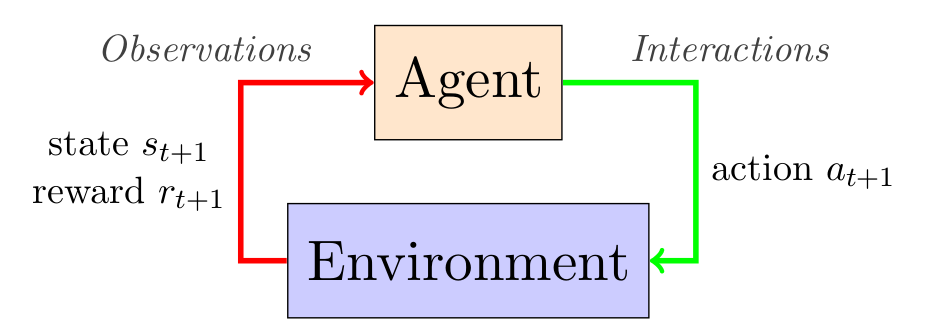
\includegraphics[scale=0.4]{figures/agentenvironment.png}
% \caption{The agent-environment interaction in reinforcement learning}
% \label{fig:frames}
% \end{figure}

\begin{figure}[H]
\centering
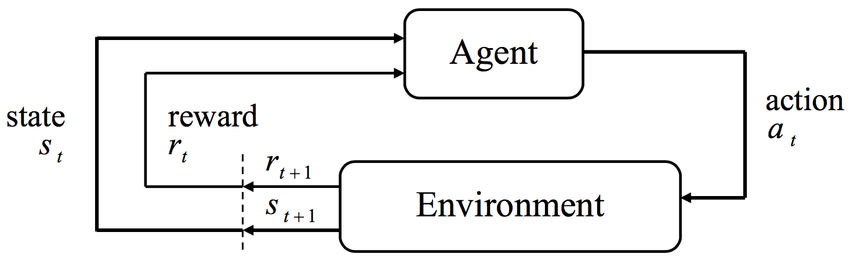
\includegraphics[scale=0.25]{figures/agenv.png}
\caption{The agent-environment interaction in reinforcement learning}
\label{fig:ageenv}
\end{figure}
% Some of the key RL applications are:
% \begin{enumerate}
% \item Allocation of limited resources(computer clusters) to different tasks as per priority.
% \item Temporal difference learning is used in high-performance Atari games.
% \item Controlling network traffic signals using a multi agent reinforcement system.
% \item Training robots to learn policies and take actions by maximizing rewards.
% \item Optimizing chemical reactions by using deep reinforcement learning.
% \end{enumerate}
In this paper various reinforcement learning algorithms are employed to solve a simulated real world problem of cab pickups and drops. The performance of agents trained using these different algorithms and the rewards obtained are evaluated and compared for analysis. The rest of the paper is organised as follows: \hyperref[sec:2]{Section 2} reviews the related work in the domain. We defined the problem and the algorithms used in \hyperref[sec:3]{Section 3}. \hyperref[sec:4]{Section 4} discusses the experimental results and evaluation. Finally, \hyperref[sec:5]{Section 5} gives the concluding remarks.
 

\section{Related Work}
\label{sec:2}
Osmankovic et al. \cite{osmankovic2011implementation} introduce the concept of Q-Learning as the quintessential algorithm to solve a-typical ‘maze’ problems using reinforcement learning. The paper highlights an action-reward methodology where the agent’s actions are determined based on a knowledge-matrix that is iteratively updated. The methodology suffers the drawback of only utilizing the knowledge matrix to pick future actions, consequently, not allowing the agent to explore the state space.

Kantasewi, Marukatat et al. \cite{kantasewi2019multi} approaches the same version of this problem with a more robust approach. They involve multiple knowledge matrices from which the agent learns iteratively about its environment with an aim to increase its overall reward score. The methodology proposed involves a dynamic $\epsilon$ value, which is initially initialized as a high value, and keeps reducing based on the agent’s learned actions to provide a balance between ‘exploration’ and ‘exploitation’. Our project includes an extension of this methodology.

In \cite{lin2019solving}, Shih-Wei Lin compared three reinforcement learning (RL) algorithms to solve a maze problem by exploring the moving mode of mobile robot path planning. These three RL algorithms are Random Algorithm, Strategy Gradient Algorithm and SARSA (State Action Reward State Action). The best advantage of RL is that in the learning process, there is no right response except learning by reward messages. 

% The RL system's learning target is reward, the learning source is the technique and the total benefit is maximized by maximizing technique. In other words, the task of reinforcement learning is to learn the mapping of the environment to the action.

Mnih et al. \cite{mnih2013playing} demonstrated deep Q-Network (DQN), a novel reinforcement learning agent that uses a Convolutional Neural Network (CNN) as a non-linear function approximator for the action-value (also known as Q) function in Q-learning. The DQN agent was tested across 49 tasks from the Atari 2600 platform and was shown to outperform the best existing reinforcement learning method in 43 tasks while also delivering comparable performance to a professional human games tester across all 49 tasks \citep{mnih2015human}.

% The DQN agent used the same network architecture and hyperparameters for all the tasks, thus demonstrating how advances in deep neural networks could be used in reinforcement learning to perform a variety of tasks with minimal prior knowledge.  




\section{Problem Definition and Algorithms}
\label{sec:3}
We address the Taxi problem using the OpenAI Gym toolkit \citep{knuthwebsite}. There are six primitive actions and 500 state spaces in this environment. These include four navigation actions that move the taxi one square either North, South, East or West and pickup and dropoff. There are 4 possible pickup and drop positions (R,G,B,Y) as shown in Figure \ref{fig:frames}. The current pickup and drop locations are displayed in Blue and Purple respectively. There is a reward of -1 for each action and an additional reward of +20 for successfully delivering the passenger. There is a reward of -10 if the taxi attempts to execute the drop or pickup actions illegally. The taxi problem requires an algorithm that supports temporal abstraction, state abstraction and subtask sharing which makes Reinforcement learning an ideal candidate for solving the task \citep{dietterich2000hierarchical}.
\begin{figure}[H]
\centering
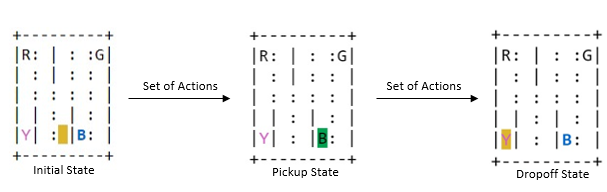
\includegraphics{figures/frames.png}
\caption{Frames depicting environment states}
\label{fig:frames}
\end{figure}
To create a baseline we have attempted to solve the problem using ‘Random Search’, followed by various state-of-the-art algorithms with a collection of hyperparameter values to measure individual algorithm performance over a range of parameters.


\subsection{Random Search}
Random Search \citep{spitzer2013principles} also known as Random Walk is a local search technique that determines random paths to achieve the end goal of a problem comprising multiple actions and states. In Random Search Algorithm, we start at a given initial state, choose a random action from the available actions, transit to the next state; and then keep doing the same until the goal is reached. Which action the agent should choose can also be determined using probability distribution after running the algorithm multiple times to solve a specific problem and recording the observations. Its pseudo-code is given below.

\begin{algorithm}
\caption{Random Search}
\begin{algorithmic}[1]
\REQUIRE  Initial State S, Terminal State T and all available actions A
\STATE Initialize $current\_state \leftarrow S$
\REPEAT
\STATE Choose a random action $a \in $A 
\STATE  Observe and record reward R
\STATE Transit to $next\_state  \leftarrow $S'
\STATE Update $current\_state \leftarrow $next\_state
\UNTIL{$current\_state  \neq  T$}
\end{algorithmic}
\end{algorithm}


The algorithm is easy to understand and implement as it does not require any domain specific knowledge and hyperparameters. Owing to its nature, it works well for problems with a small number of possible states/ search space. Since the next action is selected at random and independent of the previous state, there is no need to save the states in the memory. This makes it memory efficient. For complex problems, which requires high computation to determine the next best possible action can leverage the use of Random Search Algorithm to overcome the computation limitations of the agent.
The algorithm is asymptotically complete, however does not guarantee an optimal solution.  

\subsection{Q-Learning}
The Q-Learning algorithm is an iterative offline learning algorithm where the environment’s agent learns from the rewards and penalties it receives from the environment as it proceeds to achieve its target state. The algorithm maintains a global knowledge matrix Q-table containing these state-action value pairs can be denoted as Q(state,action). The Q-table is initialized to all zeros before training begins, and is iteratively updated using the following formula: \\

   Q(state, action) \leftarrow Q(state, action) + (reward + max Q(next state,action space)) \\

Where, $\alpha$ is the learning rate parameter and 0 $<$ $\alpha$ $\leq$ 1. The parameter $\gamma$ defines the discount level and 0 $\leq$ $\gamma$ $\leq$ 1. A high value for this parameter indicates that the agent should consider the long term benefits of an action instead of the short term benefits and vice versa. The importance of this parameter is that it enables the agent to select the shortest path to achieve its goal while minimising penalties. The algorithm essentially employs a ‘look-ahead’ approach as the Q-table is updated with the sum of the weighted value of the current state i.e. Q(state, action), with the sum of the reward received for taking the current step and the discounted maximum reward we might receive by taking the next step i.e. reward + max Q(next state,action space). Therefore we are always considering the step that has the maximum learned value in the knowledge matrix. 

There are two ways for the agent to select an action at each iteration. To maintain an effective balance between exploitation and exploration a third parameter is introduced - $\epsilon$ where 0 $\leq$  $\epsilon$ $\leq$ 1. A smaller value of $\epsilon$ allows the agent to explore where we allow the agent to sample an action at random from the environment, this helps the agent to learn the environment surroundings, while a larger value allows the agent to be greedy and pick actions from the learned table that has the maximum value for that particular state. 
To attain a balance the $\epsilon$-greedy approach is introduced. The pseudo-code including all parameters are as follows:

\begin{algorithm}
\caption{Q-Learning}
\begin{algorithmic}[1]
\REQUIRE Initial State S, Terminal State T, all available actions A, Q-table Q(s,a) for all state-action pairs $\mid$ s $\in$ S and a $\in$ A , $\alpha$, $\gamma$, $\epsilon$
\STATE Initialize $current\_state \leftarrow  S$
\REPEAT
\IF  {unif(0,1) $<$ $\epsilon$}
\STATE $action$ $\leftarrow$ sample action from environment
\ELSE
\STATE $action$ $\leftarrow$ $max\_action(Q(current\_state)$
\ENDIF
\STATE $next\_state$ , $reward$ , $final\_state$ $\leftarrow$ result of action on environment
\STATE $current\_value$ $\leftarrow$ $Q(state,action)$
\STATE $next\_value$ $\leftarrow$ $max(Q(next\_state))$
\STATE $Q(state,action)$ $\leftarrow$ (1 - $\alpha$) * $current\_value$ + $\alpha$ * ($reward$ + $\gamma$ * $next\_value$)
\STATE Update $current\_state$ $\leftarrow$ $next\_state$
\UNTIL{$current\_state  \neq  T$}
\end{algorithmic}
\end{algorithm}

\subsection{SARSA (State Action Reward State Action)}
The SARSA algorithm proposed in \citep{sutton1996generalization,sutton1988learning}, is an improved Q-learning algorithm. The SARSA method estimates the value of Q(st,at) by applying at in state s(t) according to the following updated formula: \newline

Q(S,A) \leftarrow Q(S,A) +  ($\alpha$)[R + $\gamma$ * Q(S',A') - Q(S,A)] \\ \\
This update is done after every transition from a nonterminal state st. Q(st+1,at+1) is defined as zero if st+1 is terminal. SARSA is an on-policy TD control method. A policy calculates the action taken on each state based on the maximum reward by estimating Q(s,a).If a state S is terminal (goal state or end state) then, Q (S, a) = 0 $\forall$ a $\in$ A where A is the set of all possible actions. \newline
Action is chosen as per Epsilon-greedy policy:
\begin{enumerate}
    \item Generate a random number r $\in$ [0,1].
    \item If r $<$ $\epsilon$ choose an action derived from the Q values (which yields the maximum reward).
    \item Else choose a random action.
\end{enumerate}


\begin{algorithm}
\caption{SARSA}
\begin{algorithmic}[1]
\REQUIRE Initial State S, Terminal State T, all available actions A, Q-table Q(s,a) for all state-action pairs $\mid$ s $\in$ S and a $\in$ A , $\alpha$, $\gamma$, $\epsilon$
\STATE Initialize $current\_state \leftarrow  S$
\STATE Choose $current\_action$  from $S'$ using epsilon greedy policy Q
\REPEAT
\STATE $action a$ $\leftarrow$ sample action from environment
\STATE Take action $a$, observe reward $R$ , $next\_state \leftarrow S'$
\STATE Choose $a'$ (next action) from $S'$ using epsilon greedy policy Q
\STATE $Q(S,a)$ $\leftarrow$  $Q(S,a)$ +  ($\alpha$)[R + $\gamma$ * $Q(S',a')$ - $Q(S,a)$]
\STATE Update $current\_state$ = $next\_state$
\UNTIL{$current\_state  \neq  T$}
\end{algorithmic}
\end{algorithm}

\newpage
\subsection{Expected-SARSA}
 Expected SARSA is a variance of Q-Learning. Expected-SARSA is an on-policy algorithm since it updates its Q-values using the Q-value of the next state $s'$ and the current policy's action $a''$. Expected SARSA selects the output of a state not on the Q-value but instead on the expected Q-value. The benefit of choosing the expected Q-value is that we reduce variance in the update from state to state. Having a lower variance means that we can increase $\alpha$ so that our algorithm learns faster. SARSA requires an \newline $\alpha$ $<$ 1 while Expected-SARSA can have $\alpha$ = 1. Since Expected-SARSA can take action-selection after the update, this is advantageous for returning actions such as what occurs in Taxi-v3. Importantly, Expected-SARSA has the same convergence guaranteed \citep{van2009theoretical} as SARSA and thus can reach the optimal policy in the limit.
\newline
The hyperparameters for Expected-Sarsa are alpha, gamma, epsilon start, epsilon decay and epsilon cut. Choosing the right hyperparameters is important in reaching the highest reward possible. Alpha ($\alpha$) is the most important hyperparameter. It affects how fast the algorithm converges but comes at a cost of a lower reward.

\begin{algorithm}[h]
\caption{Expected-SARSA}
\begin{algorithmic}[1]
\REQUIRE Initial State S, Terminal State T, all available actions A,Q-table Q(s,a) for all state-action pairs $\mid$ s $\in$ S and a $\in$ A , $\alpha$, $\beta$, $\gamma$
\STATE Initialize $current\_state \leftarrow  S$
\REPEAT
\STATE Choose $current\_action$ $\leftarrow$ $a$  from state using policy $\pi$ derived from Q
\STATE Take action $a$, observe reward $R$ , $next\_state \leftarrow S'$
\STATE $Vs'$ $\leftarrow$ $\sum$ $\pi(S', a) * Q(S', a)$
\STATE $Q(S,a)$ $\leftarrow$  $Q(S,a)$ +  ($\alpha$) * [R + $Vs'$ * $Q(S',a')$ - $Q(S,a)$]
\STATE Update $current\_state$ = $next\_state$
\UNTIL{$current\_state  \neq  T$}
\end{algorithmic}
\end{algorithm}


\subsection{Deep Q-Learning}
The algorithm used to train a deep Q-network has been described as a variant of the Q-learning algorithm in the original research paper. Q-learning selects optimal actions at each time-step using the action-value (also known as Q) function. The optimal Q-function follows an identity known as a \textit{Bellman Equation} which is shown below.
\begin{equation}
    Q^{*}(s,a) = E_{s'\sim\varepsilon}[r + \gamma \max_{a'}Q^{*}(s',a')| s,a]
\end{equation}
Reinforcement learning algorithms estimate the Q-function using an iterative update \(Q_{i+1}(s,a)=E_{s'\sim\varepsilon}[r + \gamma \max_{a'}Q_{i}(s',a')| s,a] \). The Deep Q-Learning algorithm uses a Convolutional Neural Network (CNN) to estimate the Q function, \(Q(s,a;\theta)\approx Q^{*}(s,a) \), which is also known as a Q-network. A Q-network is trained by minimising the loss function, 
\begin{equation}
   L_{i}(\theta_{i})=E_{s,a\sim\rho(.)}[(y_{i}-Q(s,a;\theta_{i})^2] 
\end{equation}
at each iteration i, where \(y(i)= E_{s'\sim\varepsilon}[r + \gamma \max_{a'}Q(s',a';\theta_{i-1})| s,a]\) is the target for iteration i. The weights of the Q-network are updated using stochastic gradient descent. Reinforcement learning algorithms have been known to be unstable with non-linear function approximators. To tackle this, the Deep-Q Learning algorithm uses Experience Replay \citep{lin1993reinforcement}, i.e., randomly sampling from past observations to reduce correlations in the training data. Pseudo-code below:
% Also, the Q-network is updated towards the target in each iteration.
% To estimate the target, another Q-network called the target network is used, whose parameters are cloned from the original network periodically. This is done to remove correlations of q-values with the target. The Deep Q-learning algorithm is shown (Algorithm 5).

\begin{algorithm}
\caption{Deep Q-Learning with Experience Replay}
\begin{algorithmic}
\STATE Initialize replay memory \(D\) to capacity \(N\)
\STATE Initialize action-value function \(Q\) with random weights \(\theta \)
\STATE Initialize target action-value function \(\hat{Q}\) with weights \(\theta^{-}=\theta \)
\FOR{$episode=1,M$}
% \STATE Initialize sequence \(s_{1}=\{x_1\}\) and preprocessed sequence \(\phi_{1}=\phi(s_1)\)
\FOR{$t=1,T$}
\STATE With probability \(\epsilon\) select a random action \(a_t\)
\STATE otherwise select \(a_{t}=argmax_{a}Q(s_t,a;\theta)\)
\STATE Execute action \(a_t\) and observe reward \(r_t\) and state \(s_{t+1}\)
\STATE Store transition \((s_{t}, a_{t}, r_{t}, s_{t+1})\) in \(D\)
\STATE Sample random minibatch of transitions \((s_{j},a_{j},r_{j},s_{j+1})\) from \(D\)
\STATE Set \[ y_j = \begin{cases}
r_j & \text{ if episode terminates at step } j+1 \\
r_j+\gamma \max_{a'}\hat{Q}(s_{j+1},a';\theta^{-}) & \text{ otherwise }
\end{cases} \]
\STATE Perform a gradient descent step on \((y_{j}-Q(s_{j},a_{j};\theta))^2\) with respect to the network parameters \(\theta\)
\STATE Every \(C\) steps reset \(\hat{Q}=Q\)
 \ENDFOR
\ENDFOR
\end{algorithmic}
\end{algorithm}

% The original algorithm was configured for Atari 2600 games and received successive frames (static images) of the game as input and used a CNN for the Q-network. We modify the algorithm to take as input a one-hot vector representing one of 500 possible states of the taxi environment. As the input is a 1-D vector, we use linear feed-forward layers instead of convolutional layers. Our implementation contains 1 hidden layer of 150 neurons as well as a Dropout layer. The original paper used RMSProp as the Optimizer for the neural network whereas we used the Adam Optimizer.


\newpage
\section{Experimental Results}
\label{sec:4}
The agent is trained with 5000 iterations or episodes using the each of algorithms described above. A single iteration in the experiment consists of certain epochs, which is the number of time-steps the agent took to reach the final state from the initial state, and a penalty count. The penalty count is the number of times the agent incurred a reward = -10. The observations of averaging over 5000 iterations are recorded in a table x, and individual algorithm performances are shown in Figure \ref{fig:comparativeplot}. The algorithms are tested with a collection of hyperparameter values as shown in \hyperref[tab:table]{Table 1}.


\subsection{Random Search}
Random search is applied to the problem to create a baseline performance for reinforcement learning algorithms mentioned above. The graph (Figure \ref{fig:comparativeplot}) is plotted which shows the total penalty count incurred by the agent for each iteration. As evident from the graph, the performance of the agent does not improve with iterations unlike RL algorithms. The reason being that the agent does not learn from its previous actions and the environment. Hence, it takes a very large number of steps to reach the terminal state.

\subsection{Q-Learning}
The Q-Learning is applied is to the problem and values of learning parameters are varied to study how agents behave in different situations. The experimentation produced distinguishable results for $\alpha$ = 0.1 and 0.4, $\gamma$ = 0.6 and 0.9. It is evident from Figure \ref{fig:comparativeplot} that the exploiting ($\epsilon$ = 0.9) the learned values helped the agent converge faster and steadily as compared to exploring ($\epsilon$ = 0.1) and balanced ($\epsilon$ = 0.5) approaches. Also the latter combinations of $\alpha$ and $\gamma$ were found to be more effective in almost all algorithms.

\subsection {SARSA}
SARSA algorithm applied to the problem involved comparison of the outcomes using different parameter values of $\alpha$, $\gamma$ and $\epsilon$. Different values of $\epsilon$ used are 0.9 (Exploitation), 0.1 (Exploration) and 0.5 (Less extreme). For parameter values of $\alpha$ = 0.1 and $\gamma$ = 0.6, Q-learning performed better than SARSA as it took more epocs to converge with high penalty. On the other hand, SARSA outperformed Q-learning for parameter values of $\alpha$ = 0.4 and $\gamma$ = 0.999 as evident from Figure \ref{fig:comparativeplot}.

\subsection{Expected-SARSA}
Another algorithm used to solve the problem is Expected-SARSA. As per the algorithms before, the hyperparameters $\alpha$, $\gamma$ and $\epsilon$ are varied and the convergence and number of penalties are monitored. As seen in Figure \ref{fig:comparativeplot} the algorithm has wild fluctuations at the start before stabilizing steadily to converge. This shows that the initialization of the $\alpha$ has a profound impact on the stability of the Expected-SARSA algorithm. We can also observe from \hyperref[tab:table]{Table 1} that the $\alpha$ = 0.4 configurations have nearly 50\% less penalties than when $\alpha$ = 0.1. Finally, when comparing the average epochs and average penalties of Expected-SARSA with SARSA and Q-Learning we can see that Expected-SARSA has the lowest number of penalties incurred. 

\subsection{Deep Q-Learning}
The Deep Q-learning algorithm applied to solve the problem takes as input a one-hot vector representing one of 500 possible states of the taxi environment. Since the input is a 1-D vector, linear feed-forward layers are used instead of convolutional layers. The implementation contains 1 hidden layer of 150 neurons as well as a Dropout layer. Its performance is depicted in Figure \ref{fig:comparativeplot}.
% \newpage
\begin{figure}[]
\centering
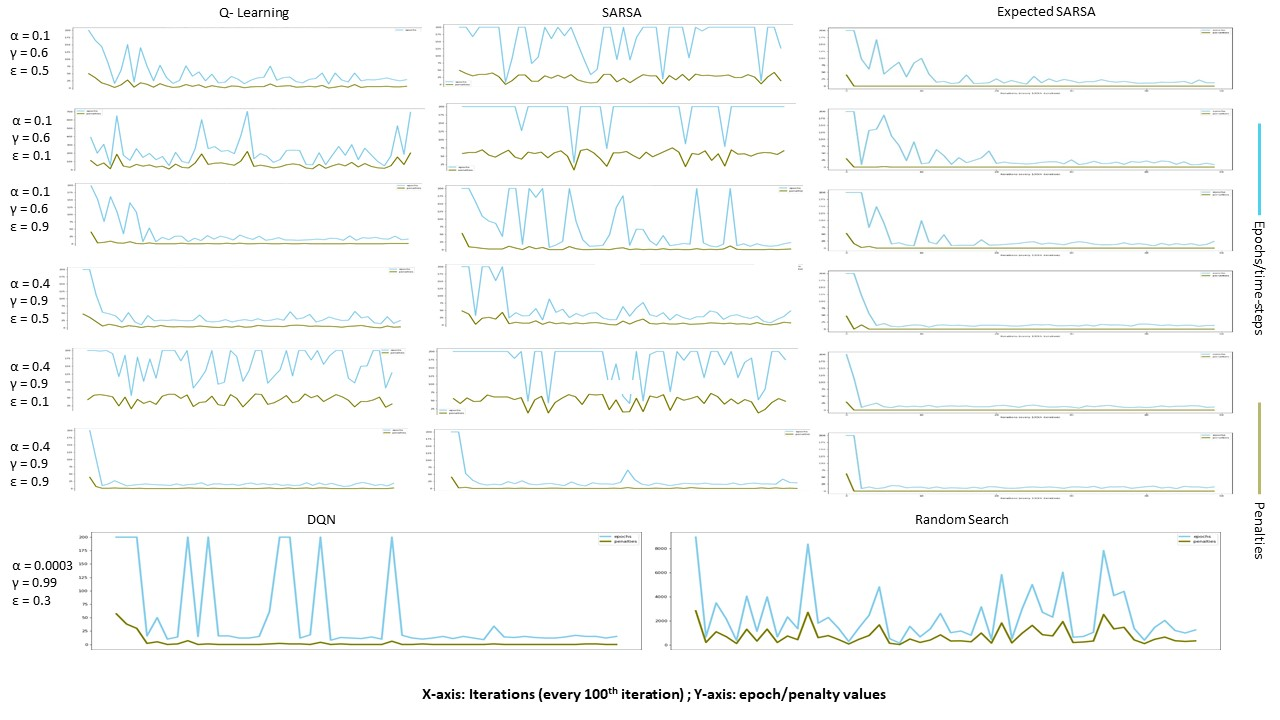
\includegraphics[scale = 0.4]{figures/comparativeplotFinal.jpg}
\caption{Performance Graphs: Iterations vs Epocs }
\label{fig:comparativeplot}
\end{figure}


% \begin{figure}[h]
% \centering
% 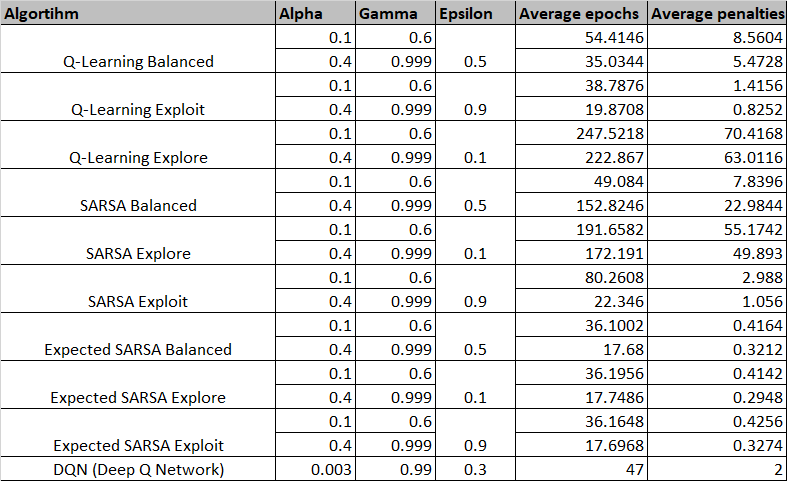
\includegraphics[scale=0.65]{figures/table.png}
% \caption{Performance Graphs: Iterations vs Epocs }
% \label{tab:table}
% \end{figure}

% \begin{table}[H]
% \centering
% 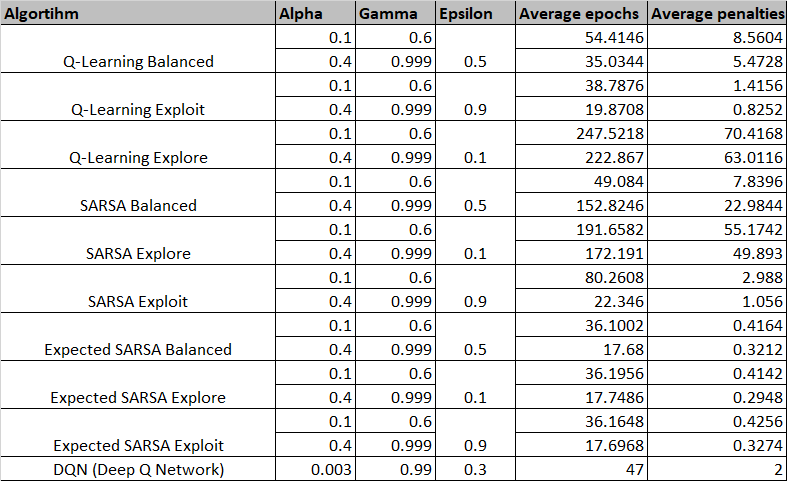
\includegraphics[scale=0.65]{figures/table.png}
% \caption{Results observed for algorithms for different values of hyperparameters} 
% \label{tab:comparison}
% \end{table}

% Please add the following required packages to your document preamble:
% \usepackage{booktabs}
% \usepackage{multirow}
\begin{table}
% \caption{Results observed for algorithms for different values of hyperparameters} 
\setlength{\tabcolsep}{4pt}
\begin{tabular}{@{}lrrrrr@{}}
\toprule
Algorithm                                & Epsilon              & Alpha & Gamma & Average Epochs & Average Penalties \\ \midrule
\multirow{Q-learning Balanced}     & \multirow{0.5} & 0.1   & 0.6   & 54.4146        & 8.5604            \\\addlinespace[0.2em]
                                         &                      & 0.4   & 0.999 & 35.0344        & 5.4728            \\\addlinespace[0.2em]
\multirow{Q-learning Exploit}      & \multirow{0.9} & 0.1   & 0.6   & 38.7876        & 1.4156            \\\addlinespace[0.2em]
                                         &                      & 0.4   & 0.999 & 222.867        & 63.0116           \\\addlinespace[0.2em]
\multirow{Q-learning Explore}      & \multirow{0.1} & 0.1   & 0.6   & 247.5218       & 70.4168           \\\addlinespace[0.2em]
                                         &                      & 0.4   & 0.999 & 222.867        & 63.0116           \\\addlinespace[0.2em]
\multirow{SARSA Balanced}          & \multirow{0.5} & 0.1   & 0.6   & 49.084         & 7.8396            \\\addlinespace[0.2em]
                                         &                      & 0.4   & 0.999 & 152.8246       & 22.9844           \\\addlinespace[0.2em]
\multirow{SARSA Exploit}           & \multirow{0.9} & 0.1   & 0.6   & 80.2608        & 2.988             \\\addlinespace[0.2em]
                                         &                      & 0.4   & 0.999 & 22.346         & 1.056             \\\addlinespace[0.2em]
\multirow{SARSA Explore}           & \multirow{0.1} & 0.1   & 0.6   & 191.6582       & 55.1742           \\\addlinespace[0.2em]
                                         &                      & 0.4   & 0.999 & 172.191        & 49.893            \\\addlinespace[0.2em]
\multirow{Expected SARSA Balanced} & \multirow{0.5} & 0.1   & 0.6   & 36.1002        & 0.4164            \\\addlinespace[0.2em]
                                         &                      & 0.4   & 0.999 & 17.68          & 0.3212            \\\addlinespace[0.2em]
\multirow{Expected SARSA Exploit}  & \multirow{0.9} & 0.1   & 0.6   & 36.1648        & 0.4256            \\\addlinespace[0.2em]
                                         &                      & 0.4   & 0.999 & 17.6968        & 0.3274            \\\addlinespace[0.2em]
\multirow{Expected SARSA Explore}  & \multirow{0.1} & 0.1   & 0.6   & 36.1956        & 0.4142            \\\addlinespace[0.2em]
                                         &                      & 0.4   & 0.999 & 17.7486        & 0.2948            \\\addlinespace[0.2em]
DQN (Deep Q Network)                     & 0.3                  & 0.3   & 0.99  & 47             & 2                 \\ \bottomrule
\end{tabular}
\label{tab:table}
% \caption{Results observed for algorithms for different values of hyperparameters} 
\end{table}
% \begin{table*}[bp]
% \centering
% \begin{tabular}{@{}rrrrrrrrr@{}}\toprule
% &\multicolumn{2}{c}{$Algorithm$} &{$Alpha$} & {$Gamma$} & {$Epsilon$} & {$Average Epochs$} & {$Average Penalties$}\\
% \midrule
% $MovieLens 100K$\\
% $RMSE$ & $0.8758$ & $\textbf{0.8666}$ & $1.04885$ & $0.9526$ & $0.9683$ & $0.8957$ & $1.2652$ & $1.8310$\\
% $MAE$ & $0.7733$ & $0.7083$ & $0.7482$ & $0.6840$ & $0.9848$ & $1.4884$ & $\textbf{0.6740}$ & $0.6755$\\\\

% $Last.fm$\\

% $RMSE$ \\
% $MAE$ \\
% \bottomrule
% \end{tabular}
% \caption{Auto-CaseRec Evaluation Results}
% \end{table*}

% \begin{itemize}
% \item Methodology: describe the evaluation criteria, the data used during the evaluation, and the methodology followed to perform the evaluation. 
% \item Results: present the results of the experimental evaluation. Graphical data and tables are two common ways to present the results. Also, a comparison with a baseline should be provided.
% \item Discussion: discuss the implication of the results of the proposed algorithms/models. What are the weakness/strengths of the method(s) compared with the other methods/baseline?
% \end{itemize}

\newpage
\section{Conclusions}
\label{sec:5}
Our comparative analysis led us to believe that the Expected-SARSA algorithm worked best giving the least average time steps for the agent to reach its final destination, followed by Q-Learning, DQN and SARSA. Comparing these state-of-the-art algorithms with our baseline Random Search results clearly shows immense improvement. Moreover, it can also be observed better results are achieved using the exploitation approach as compared to the exploration. Thus, it is prudent to give more weightage to the iteratively learned values as compared to letting the agent explore the environment.

\bibliographystyle{ieeetr}
\bibliography{mybib}

% \begin{thebibliography}{6}


% \bibitem {smit:wat}
% Smith, T.F., Waterman, M.S.: Identification of common molecular subsequences.
% J. Mol. Biol. 147, 195?197 (1981). \url{doi:10.1016/0022-2836(81)90087-5}

% \bibitem {may:ehr:stein}
% May, P., Ehrlich, H.-C., Steinke, T.: ZIB structure prediction pipeline:
% composing a complex biological workflow through web services.
% In: Nagel, W.E., Walter, W.V., Lehner, W. (eds.) Euro-Par 2006.
% LNCS, vol. 4128, pp. 1148?1158. Springer, Heidelberg (2006).
% \url{doi:10.1007/11823285_121}

% \bibitem {fost:kes}
% Foster, I., Kesselman, C.: The Grid: Blueprint for a New Computing Infrastructure.
% Morgan Kaufmann, San Francisco (1999)

% \bibitem {czaj:fitz}
% Czajkowski, K., Fitzgerald, S., Foster, I., Kesselman, C.: Grid information services
% for distributed resource sharing. In: 10th IEEE International Symposium
% on High Performance Distributed Computing, pp. 181?184. IEEE Press, New York (2001).
% \url{doi: 10.1109/HPDC.2001.945188}

% \bibitem {fo:kes:nic:tue}
% Foster, I., Kesselman, C., Nick, J., Tuecke, S.: The physiology of the grid: an open grid services architecture for distributed systems integration. Technical report, Global Grid
% Forum (2002)

% \bibitem {onlyurl}
% National Center for Biotechnology Information. \url{http://www.ncbi.nlm.nih.gov}


% \end{thebibliography}

\end{document}
